%%%%%%%%%%%%%%%%%%%%%%%%%%%%%%%%%%%%%%%%%%%%%%%%%%%%%%%%%%%%%%%%%%%%%%%%%%%%%%%%
%2345678901234567890123456789012345678901234567890123456789012345678901234567890
%        1         2         3         4         5         6         7         8
%
% Slightly modified by X. Baró for FG2020
%

%\documentclass[letterpaper, 10 pt, conference]{ieeeconf}  % Comment this line out
% if you need a4paper
\documentclass[a4paper, 10pt, conference]{ieeeconf}      % Use this line for a4
\usepackage{float}                                                            % paper
\usepackage{FG2020}

%\FGfinalcopy % *** Uncomment this line for the final submission
\usepackage{multicol}

\IEEEoverridecommandlockouts                              % This command is only
% needed if you want to
% use the \thanks command
\overrideIEEEmargins
% See the \addtolength command later in the file to balance the column lengths
% on the last page of the document

% The following packages can be found on http:\\www.ctan.org
%\usepackage{graphics} % for pdf, bitmapped graphics files
%\usepackage{epsfig} % for postscript graphics files
%\usepackage{mathptmx} % assumes new font selection scheme installed
%\usepackage{times} % assumes new font selection scheme installed
%\usepackage{amsmath} % assumes amsmath package installed
%\usepackage{amssymb}  % assumes amsmath package installed
\newenvironment{tablehere}
\usepackage{indentfirst}
\setlength{\parindent}{2em}
\usepackage{graphics} % for pdf, bitmapped graphics files
\usepackage{epsfig} % for postscript graphics files
\usepackage{mathptmx} % assumes new font selection scheme installed
\usepackage{times} % assumes new font selection scheme installed
\usepackage{amsmath} % assumes amsmath package installed
\usepackage{amssymb}  % assumes amsmath package installed
\usepackage{multirow}
\usepackage{caption}

\def\FGPaperID{****} % *** Enter the FG2020 Paper ID here

\title{\LARGE \bf Pseudo-Convolutional Policy Gradient for Sequence-to-Sequence Lip-Reading
}

%use this in case of a single affiliation
%\author{\parbox{16cm}{\centering
%    {\large Huibert Kwakernaak}\\
%    {\normalsize
%    Faculty of Electrical Engineering, Mathematics and Computer Science, University of Twente, Enschede, The Netherlands\\}}
%    \thanks{This work was not supported by any organization.}% <-this % stops a space
%}

%use this in case of several affiliations
\author{\parbox{16cm}{\centering
		{\large Huibert Kwakernaak$^1$ and Pradeep Misra$^2$}\\
		{\normalsize
			$^1$ Faculty of Electrical Engineering, Mathematics and Computer Science, University of Twente, Enschede, The Netherlands\\
			$^2$ Department of Electrical Engineering, Wright State University, Dayton, USA}}
	\thanks{This work was not supported by any organization}% <-this % stops a space
}

\usepackage[normalem]{ulem} % use normalem to protect \emph %DIF > 
\newcommand\hl{\bgroup\markoverwith {\textcolor{yellow}{\rule[-.5ex]{2pt}{2.5ex}}}\ULon}
\begin{document}
	
	\ifFGfinal
	\thispagestyle{empty}
	\pagestyle{empty}
	\else
	\author{Anonymous FG2020 submission\\ Paper ID \FGPaperID \\}
	\pagestyle{plain}
	\fi
	\maketitle
	
	
	
	%%%%%%%%%%%%%%%%%%%%%%%%%%%%%%%%%%%%%%%%%%%%%%%%%%%%%%%%%%%%%%%%%%%%%%%%%%%%%%%%
	\begin{abstract}
		Lip-reading aims to infer the speech content from the lip movement sequence, and can be seen as a typical sequence-to-sequence (seq2seq) problem which translates the input image sequence of lip	movements to the text sequence of the speech content.
		% 
		However, the traditional learning process of the seq2seq models always suffers from two problems: the exposure bias resulted by the strategy of ``teacher-forcing", and the inconsistency between the discriminative optimization target (usually the cross-entropy loss) and the final evaluation metric (usually the word error rate), leading to inferior perofrmance even when using the optimized trained model. 
		% 
		In this paper, we introduce reinforcement learning (RL) to address these two problems. Specifically, we introduce the evaluation metric as a form of reward to optimize the model together with the original discriminative target. Inspired by the local perception, weight sharing and many other appealing properties of the convolutional operation, we propose a pseudo-convolutional policy gradient based seq2seq model to take more context around each time step into account, leading to a robust reward and loss at each time-step. This step performs like imposing the convolutional operation on the reward and loss in the temporal dimension. % and so leads to our pseud-convolutional policy gradient (PCPG) method. 
		% 两种写法:
		% 一种是受conv启发,提出了一种pseudo-convolutional ..., 但这时候要讲明白为什么不能直接用conv?
		% 第二种是说提出了一种pseudo-convolutional xxx,它和conv有什么共同点,所以称为pseudo-conv...
		% 先遗留,看完正文后,再看具体哪种写法更合适
		%Compared with the traditional seq2seq learning process, the proposed pseudo-convolutional policy gradient (PCPG) can make good use of both the history and the future reward, and in the meanwhile is able to extend the receptive field of the reward at each time-step, contributing to improve the robustness of the model. 
		We evaluate our method on both the large-scale word-level and sentence-level benchmarks which contain a wide variety of speech conditions. With a thorough comparison and analysis, our results show either a new state-of-the-art performance or a competitive accuracy on these challenging benchmarks, which clearly demonstrate the effectiveness of our approach.
	\end{abstract}
	
	
	%%%%%%%%%%%%%%%%%%%%%%%%%%%%%%%%%%%%%%%%%%%%%%%%%%%%%%%%%%%%%%%%%%%%%%%%%%%%
	\section{INTRODUCTION}
	Lip-reading is an appealing manner for intelligent human-computer interaction and is receiving increasing attention in recent years. It aims to infer the speech content by using the visual information \cite{B2017} like the lip movements, and so is robust to the ubiquitous acoustic noises, making it being an important role as the complement of the audio-based speech recognition (ASR) systems, especially in a noisy environment. At the same time, lip-reading is also crucial for several other potential applications such as transcribing and re-dubbing archival silent films, sound-source localization, liveness verification and so on \cite{Chung}. 
	
	Benefiting from the vigorous development of deep learning (DL) and the emergence of several large-scale lip-reading datasets, such as GRID \cite{cooke2006}, LRW \cite{B2017}, LRW-1000 \cite{Yang2019}, LRS \cite{Chung} and so on, lip-reading has made great progresses over the past two years.
	% In summary, three main pipelines have emerged to solve the lip-reading problem. One is based on directly classify the whole image sequence into some category which is always corresponding to a word. The second one is based on the CTC loss (Connectionist Temporal Classification loss), which is often used in audio-based speech recognition systems. The last one is the seq2seq models together with the attention mechanism, which predict each character or word at each time step and is flexible for both word-level or sentence-level lip-reading task.
	%Compared with the CTC-based methods, the seq2seq based methods has canceled the independent assumption between each time step and so are more flexible. 
	%And lip-reading has a high similarity with other seq2seq tasks such as speech recognition \cite{Rohit}, machine translation \cite{IIya}, image caption \cite{Chen2017}, video caption \cite{Venugopalan}, and so on. Some seq2seq models especially encoder-decoder with attention based on RNN have been proved to be effective for these seq2seq tasks. These seq2seq models can model a strong temporal relation for the lip movement sequence and the character sequence. So the sentence or the word is also a character-level sequence. And in this way, the different lip-reading datasets can be trained with a common model.
	\begin{figure}
		\setlength{\abovecaptionskip}{0.05cm}
		\setlength{\belowcaptionskip}{-0.4cm} 
		\centering
		%\subfigure[the first subfigure]{}
		\includegraphics[width=0.47\textwidth]{images/samples.pdf}
		\caption{Examples for lip-reading. The examples in A-C are randomly sampled from the GRID, LRW and the LRW-1000 dataset, respectively.}
		\label{samples}
		\vspace{-0.5em}
	\end{figure}
	% In the meanwhile, the seq2seq based methods has canceled the independent assumption between each time step and so are more flexible compared with the CTC-based methods.
	Typicaly, lip-reading can be seen as a sequence-to-sequence (seq2seq) problem to translate the lip movement sequence to a character or word sequence, as shown in Fig. \ref{samples}. Several previous work have tried successfully to introduce seq2seq models for lip-reading \cite{Afouras2018}, \cite{Chung}, \cite{Afouras2017}, \cite{Chung2017}. %Their results on different lip reading datasets have indeed shown the advantages of seq2seq models for the lip-reading task. 
	However, most current seq2seq based methods suffer from two main drawbacks when used for the lip-reading task. 
	\textbf{The first one} is the exposure bias. Most current seq2seq models are learned with a heavy dependence on the ground-truth words at previous time-step for obtaining a correct prediction at the next time step. This approach is called ``teacher-forcing” \cite{Rennie} and used widely in lip-reading \cite{Chung2017}, \cite{Chung}, \cite{Afouras2018}. This strategy is helpful to make the model converge in a fast speed, but the optimized model learned in this way couldn't ensure the performance when used for the actual test process when there is no ground-truth and the model has to make correct prediction based on previous predictions \cite{Chopra2016}. This discrepancy would inevitably yield inaccurate results and even errors. Furthermore, this gap would make the errors accumulate quickly and make the predictions get worse along the sequence. %For example, when the condition is totally ``teacher-forcing", in this case, the teacher-forcing rate is equal to 1, we used the ground truth as the input when decoding at every time-step. 
	\textbf{The second problem} is the inconsistency between the optimized discriminative target and the final non-differentiable evaluation metric. For most lip-reading models, cross-entropy minimization (CE loss) is always applied as the optimization discriminative target, which is used at each time step to ensure the correct predictions at every time-step. This would always lead to two problems. Firstly, the optimized model may be not able to perform well when coming to test due to this inconsistency between the CE loss and the evaluation metric of WER/CER (Word/Character Error Rate). Secondly, the optimization process compute the cost at each time step independently,  giving little consideration to the predictions before and after each time-step, which could lead to the case that only a single time step or just a few time steps are predicted correctly if they have a larger loss compared with their time steps nearby.
	
	
	% The evaluation metrics for seq2seq tasks are always WER (word error rate), CER (character error rate), PER (phoneme error rate) and so on. Most of these metrics are based on an consideration of the whole sequence,
	% which are often discrete and non-differentiable, and so they are not quite fit in with the cross-entropy optimization target. 
	% 这里有两个点:(1)训练和测试不一致,一个是CE loss,一个是WER;(2)优化过程中都没有考虑context,各个time-step单独优化,有可能它自身好了,但却让别的变差了
	
	
	Inspired by the popular convolutional operations which mainly include local perception and weight sharing, we propose a new pseudo convolutional policy gradient (PCPG) based seq2seq model to solve the above two problems for robust lip-reading. On the one hand, we introduce reinforcement learning into the seq2seq model to connect the optimized discriminative target and the evaluation metric of WER/CER. On the other hand, we mimic the computation process of traditional convolutional operation to consider more time steps nearby when computing the reward and loss for each time step. By a thorough evaluation and comparison on several lip-reading benchmarks, we demonstrate both the effectiveness and the generalization ability of the proposed PCPG based seq2eq model. At the same time, we report a new state-of-the-art performance on two benchmarks and also give a competitive accuracy on another dataset.
	
	\section{Related work}
	In this section, we firstly give a survey briefly about the related work on the lip-reading task. Then we discuss the work related with the seq2seq model and reinforcement learning used in our model.
	\subsection{Lip-reading}
	Lip-reading has made several great progresses since the emergence of deep learning (DL). Many methods have been proposed based on DL \cite{Chung2018, Chung, Chung2017, B2017, Petridis2018, Assael2016, Afouras,Zhou2014, Yang2019, Hu2016}. In summary, the previous work for lip-reading can be divided into two strands according to their particular task. 
	
	The first one mainly focuses on word-level lip-reading. This type of method aims to classify the whole image sequence into a single class, no matter how many frames in the sequence. This method is proved to be effective by many previous work. For example, the work in \cite{Chung2017} proposed to extract frame-level features by the VGG network and then combine all the fratures from all the frames at several different stages to obtain the final prediction of the whole sequence. 
	In \cite{Stafylakis2017},  the authors proposed an end-to-end deep learning architecture by combining a spatiotemporal convolutional module, the ResNet module and the final bidirectional LSTM for word-level lipreading, and have obtained the state-of-the-art performance when they were published. In this paper, we would keep a similar front-end module with them and would present details in the next section. %The work in \cite{Petridis2018} presented an end-to-end audiovisual model based on residual networks and Bidirectional Gated Recurrent Units (BGRUs). And this model consisted of two streams, one for each modality, which extract features directly from mouth regions and raw waveforms. In \cite{Chung2017}, the author used multi-view datasets for lip-reading. There are some works which belong to word-level recognition are based on a softmax classifier.
	
	% \vspace{-0.02cm}
	The second strand could be easily adaptive to sentence-level lip-reading task. Different from the word-level which consider the whole image sequence as a single category, the sentence-level method has to decode the character or word at each time step to output a sentence. The LipNet model presented in \cite{Assael2016} is the first end-to-end sentence-level lip-reading model, which combined a 3-layer spatiotemporal CNN module and a 2-layer Bi-GRU network with CTC loss to obtain the sentence-level predictions. Then, the work in \cite{Afouras} evaluated not only the CTC loss, but also the beam search based process \cite{Wiseman2016} for lip-reading. All CTC based methods share an assumption that all the predictions in each time step are independent on each other and so would output the probability of each result by directly conducting product of each time step and selecting the final prediction with the maximized product. In the meantime, CTC loss has also a constraint that the length of the input image sequence has to be larger than the length of the speech content sequence. Different from the CTC based methods, seq2seq models have no such assumptions or limitations as CTC, and so begin to be used widely for lip-reading. Because in the seq2seq models, we can get any length of the output sequence without considering the length of the input sequence.
	
	% The other work is based on the LSTM based encoder-decoder architecture with attention, such in \cite{Chung}, where the model can combine the audio and visual input streams. The attention mechanism \cite{Xu2014, Vaswani2017,HIWTC2014,Parikh2016}, which is very popular recently, has become a necessary part of seq2seq models. The work in \cite{Afouras}, the authors showed three architectures: a recurrent model based on LSTMs, a fully convolutional model and the recently popular transformer model. And the authors got good performance based on the transformer model.
	%\vspace{-0.4 cm}
	\subsection{Seq2Seq models}
	In this subsection, we give a brief review about the work of seq2seq models, mainly focused on but limited to the cases for lip-reading. 
	
	Sequence-to-sequence (seq2seq) models always contain a RNN based encoder to encode the input image sequence into a vector and a RNN based decoder to predict result at each time step based on the encoder's output. In the decoding process, attention mechanism is always introduced to make the prediction operation at each output's time step being able to ``observe'' all the input sequence's time steps. As stated above, \cite{Chung, Chung2017, Afouras2018} have successfully used seq2seq models to learn the translation from the input image sequence to the text sequence. 
	% which mainly refer the models consisted of encoder and decoder based on RNN, has been more and more popular in many sequence tasks with the development of deep learning (DL) and the presence of large scale datasets these days. 
	% The encoder receives the sequence input (such as images, audios, texts) and output a single vector. The decoder receives the single vector from the encoder and produces a sequence. The seq2seq models needn't consider the length and order of the sequence. Due to these advantages, the seq2seq models have been used in many tasks and there are many works based on seq2seq models such as \cite{Sutskever2014}, \cite{Venugopalan}, \cite{Prabhavalkar2017}, \cite{Nallapati2016} and so on.
	However, the usual seq2seq models always suffer from two main limitations: the exposure bias and the metric mismatch. Firstly, the exposure bias that need ground-truth words at each time step to predict next time steo in the usual learning process, could easily lead to error accumulation along the sentence during the testing process when there are no ground-truth words available and the previous predictions are used instead.
	% For example, in the training process, the seq2seq model uses the ground truth words (or other modal data) as context while at inference the entire sequence is generated by the resulting model on its own and hence the previous words generated by the model are fed as context \cite{Zhang2019}. As a result, the predicted words at training and inference are drawn from different distributions, namely, from the data distribution as opposed to the model distribution. 
	On the other hand, most seq2seq models are optimized by minimizing the sum of the cross entropy loss at each individual time step. But when it comes to evaluation, the metrics take the whole sentence into accound with discrete and non-differentiable metrics, such as BLEU \cite{Papineni2002}, ROUGE \cite{Lin2001}, METEOR \cite{Banerjee2003}, CIDEr \cite{Tech}, WER (word error rate), CER (character error rate), SER (sentence error rate), and so on. The inconsistency between the loss and the evaluation metric could easily lead to the case that even we get a very small cross entropy loss during training, we may still not be able to get a good performance when it comes to test. %These two problems hinder the performance of seq2seq models.
	
	To address the above problems, we introduce reinforcement learning (RL) into seq2seq models for the lip readng task, as shown in Fig. \ref{overview_fig}. 
	On the one hand, the model generates the predictions at each time step based on the previous prediction results instead of the previous ground-truth words. In this way, the model can learn a stronger relationship between adjacent time steps in the output sequence than using "teacher-forcing". And so this could avoid the problem of exposure bias. 
	On the other hand, by giving appropriate rewards, we can optimize the evaluation metrics directly. To make the reward at each time step could  consider the performance around the current time step, we introduce a pseudo-convolutional policy gradient method, to mimic the local perception and weight sharing of convolution operation to enhance the contextual relevance here for robust lip-reading. Results on several different large-scale benchmarks have proved the effectiveness of our method. 
	% We introduce context around each time step together to 
	
	% For example, the work in \cite{Tjandra2017} proposed an alternative strategy for training a seq2seq ASR by  RL methods. The other work in \cite{Rennie}, based on an image caption task, proposed an optimization approach that called self-critical sequence training (SCST) and got a much better result than other ways. And specifically in \cite{Chopra2016}, Ranzato et al. used the REINFORCE algorithm \cite{Willia1992} to directly optimize non-differentiable evaluation metrics and overcome the exposure bias in different tasks (summarization, translation, image caption). However, there is no attempt to apply RL to lip-reading. And we still face some problems that how to enhance contextual relevance to get a much better generalization ability of seq2seq model, the instability and the inefficiency in the training process with RL.
	
	\begin{figure*}[htb]
		\setlength{\abovecaptionskip}{0.2cm}
		\setlength{\belowcaptionskip}{-0.3cm} 
		\centering
		%\subfigure[the first subfigure]{}
		\includegraphics[width=0.96\textwidth]{images/overall.pdf}
		\caption{Overview of our proposed PCPG based seq2seq model for lip-reading. In the model, the GRU decoder is regarded as an agent. And the ground truth is regarded as the environment. In the learning process, the agent would observe the old state generated from the previous time steps, and then takes an action to output a character/word at each current time-step to obtain a new state. The new state, the old state and the environment would together contribute to the reward for the action. Finally, the reward is feeded to the PCPG to generate the final loss when passed to the agent.}\label{overview_fig}
	\end{figure*}
	% \vspace{-0.30cm} 
	
	
	\section{The Proposed work}
	\label{sec:Pro}
	%\vspace{-0.3cm}
	In this section, we present the proposed PCPG (Pseudo-Convolutional Policy Gradient) based seq2seq model in detail. Specifically, we give the details in the order of the model's pipeline. Firstly, we describe the overall model architecture in the first subsection. Then we introduce the proposed PCPG based seq2seq model in the next subsection. Finally, we point out the differences of our work compared with the traditional methods.
	%give the reward function together with the training loss in the third subsection.
	
	\subsection{The General Model architecture} \label{section3.1}
	As shown in Fig. \ref{overview_fig}, our model can be divided into two parts: the video encoder (shown with green color) and the GRU based decoder (shown with yellow color). The video encoder part is responsible for encoding the spatiotemporal patterns in the sequence and obtain the representation of the sequence. After encoding, the GRU decoder tries to generate predictions at each time step in the principle of making the reward at each time step maximized.
	% we model the lip-reading task as a sequence-to-sequence model. The input video sequences would be decoded by the video encoder (as shown in Fig \ref{vid_encoder_fig}) into encode outputs and encoder hidden state. In the training process, we introduce the PCPG to minimize the convolutional reward-based loss. Finally, each time-step would output a character-based prediction probability, which would be used to compose and obtain the final predicted sentence or word. In the following, we would introduce the video encoder and RNN-based decoder in details. 
	
	\begin{figure}[htb]
		\setlength{\abovecaptionskip}{0.2cm}
		\setlength{\belowcaptionskip}{-0.5cm} 
		\centering
		%\subfigure[the first subfigure]{}
		\includegraphics[width=0.49\textwidth]{images/encoder.pdf}
		\caption{The CNN and RNN based video encoder. }\label{vid_encoder_fig}% consists of a Conv3d module, a Resnet18 module and a Bi-GRU module. The lip image sequence is represented by the final encoder's output and hidden state.
	\end{figure}
	\vspace{0.2cm}
	\indent{\bf The CNN and RNN based Encoder}: As shown in Fig. \ref{vid_encoder_fig}, the encoder consist of two main parts: the CNN based frontend to encode the short-term spatial-temporal patterns, and the RNN based backend to model the long-term global spatial-temporal patterns. In this part, we modified the encoder part of \cite{Wang2019} to generate the representation of the image sequence. Firstly, we apply a 3D Convolutional layer to the input image sequence to capture the initial short-term patterns in the sequence. Then a 2D convolutional encoder is followed to capture the specific movement patterns in each time step. Here, we use ResNet-18 \cite{He} as the frame-level encoder network. Finally, a 2-layer Bi-GRU is adopted to fuse these short-term and frame-level representation to a global representation of the whole sequence. We use the GRU's output $\textit{\textbf{O}}^{e}=\left(\mathbf{o}_{1}^{e}, \mathbf{o}_{2}^{e}, \dots, \mathbf{o}_{T}^{e}\right)$ and hidden-state vector $\textit{\textbf{h}}^{e}$ to record the patterns of the input video $\mathbf{X}^{v}=\left(\mathbf{x}_{1}^{v}, \mathbf{x}_{2}^{v}, \dots, \mathbf{x}_{T}^{v}\right)$, which is defined as:
	$$
	\textit{\textbf{h}}^{e}, \textit{\textbf{O}}^{e}={Encoder\_CNN\_RNN}(\mathbf{X}^{v}), \eqno{(1)}
	$$
	where $e, v, T$ denote the \textit{encoder}, the original input \textit{video} and the \textit{temporal length} of input video rerspectively.
	
	\begin{figure*}
		\setlength{\abovecaptionskip}{0.05cm}
		\setlength{\belowcaptionskip}{-0.5cm} 
		\centering
		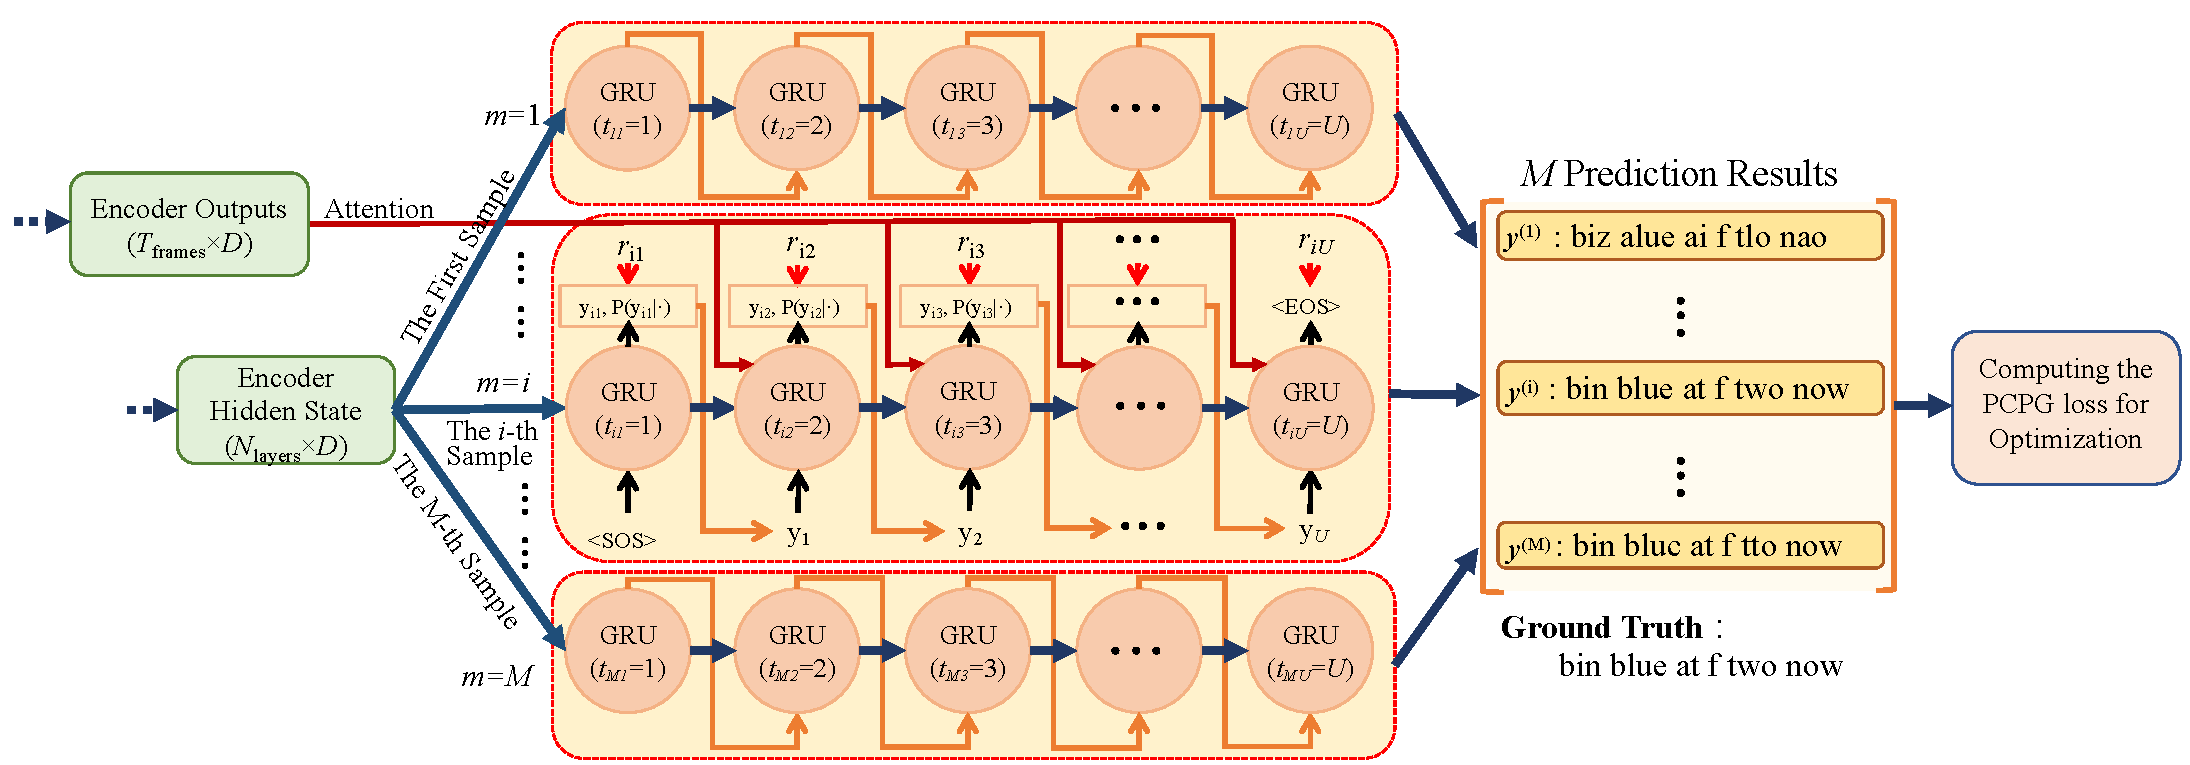
\includegraphics[width=0.98\textwidth]{images/decoder.pdf}
		\caption{Our seq2seq lip-reading decoding process with RL. The input is a sequence of frames and the output is a sequence of characters. The seq2seq model generates the target character sequence. The previous output will feedback to the agent as the next input. And the environment will feedback an immediate reward when taking an action (choosing a character at each time step). In RL, we utilize Monte Carlo sampling to sample M transcription sequences from our model to calculate the policy gradient, so we will get M output character sequences. For example, the model generates M character sequences (`biz alue ai f tlo nao', \dots, `bin blue at f two now',\dots, `bin bluc at f tto now') when the ground truth is the word ``bin blue at f two now".}\label{decoder_with_RL}
	\end{figure*} 
	
	\vspace{0.2cm}%Our PCPG based RNN decoder is shown in Fig \ref{figure3}.
	\indent{\bf The PCPG based RNN Decoder}: Given the representation of each input sequence, a 2-layer RNN is followed to decode each character at each output's tim step $u~(u=1,2,...,U)$, where $U$ denote the maximum length of the output text sequence. Our PCPG based RNN decoder is showed as Fig. \ref{decoder_with_RL}. In this paper, we use GRU as the basic RNN unit. 
	
	To learn the mutual dependencies of each output character on each time step $t$ $(t=1,2,...,T)$ in the input sequence, attention mechanism is introduced into the decoding process, which takes advantage of the context information around each time step $t$ to aid for the decoding of each output's time step $u$. With the decoder GRU's hidden state $h_{u-1}^{d}$ $(u=1,2,...,U)$ where $d$ denotes \textit{decoder}, we can compute the attention weight $\alpha_{u}$ on the current time step $u$ with respect to each input time step $t$ and the corresponding output $y_u$ at time step $u$ as 
	$$ 
	\begin{array}
	%\renewcommand{\arraystretch}{1.0}
	{c}{{e}_{u, t}=attention\left(\boldsymbol{h}_{u-1}^{d},~{o}_{t}^{v}\right) }, \\[2mm] 
	{{a}_{u, t}=\frac{e_{u,t}}{\sum_{t} e_{u,u}}}, \quad {\alpha_{u}=\sum_{t} a_{u t} o_{t}^{v}}, \\[2mm]
	\boldsymbol{y}_{u}={GRU}\left(\boldsymbol{h}_{u-1}^{d}, \boldsymbol{y}_{u}^{d},{a_{u}}\right), . 
	\end{array}
	\eqno{(2)}
	$$
	where $t=1, 2, ..., T$ and $u=1, 2, ..., U$. Finally, $(y_1, y_2, ..., y_U)$ would be used as the final output.
	
	\subsection{The PCPG based learning process}
	With the model given above, a popular way to learn the model is to minimize the cross-entropy loss  $L_{CE}$ at each time step as follows:
	% %%%%%%%%%%%%%%%%%%%%%%%%%%%%%%%%%%%%%%%%%%%%%%%%%%%%%%%%%%%%%%%%%
	% In this paper, we introduce a new reinforcement learning (RL) algorithm called PCPG for lip-reading, especially for the decoder's process. The PCPG improves the performance of the model by considering the history and future reward while general RL algorithms just only consider the future reward. And we will introduce the PCPG algorithm in details in the following sections.
	% In traditional optimization methods, we often train our models 
	% To learn the model, both the traditional cross-entropy(CE) loss and . The cross-entropy loss $L_{CE}$ is computed as following: 
	%\vspace{-0.2cm}
	$$
	{L}_{CE}=-\log p\left(c_{1}, c_{2}, \ldots, c_{U}\right)
	$$
	\vspace{-0.5cm}
	$$
	~~~~~~~~~~~~~=-\log \prod_{u=1}^{U} p\left(c_{u} | c_{1}, c_{2}, \ldots, 
	c_{u-1}\right)
	$$
	\vspace{-0.5cm}
	$$
	~~~~~~~~~~~~=-\sum_{u=1}^{U} \log p\left(c_{u} | c_{1}, c_{2}, \ldots, c_{u-1}\right). 	
	\eqno{(3)}
	$$
	where $c_{u} = 1, 2, ..., C$ is the predicted class label index at time step $u$, $C$ is the number of categories to be predicted at each time step. In this paper, There are $C = 40$ categories at each time step $u$, including $26$ alphabets, $10$ numbers, the space, the begining, padding and ending symbol. 
	
	At each time step $u$, the model would generate a prediction result according to the predictions at previous time steps $1, 2, ..., u-1$. In other words, the prediction at each time step acutally would be affected by the predictions at previous time step. At the same time, considering the bi-directional property of the Bi-GRU, we mimic the operation of 1D convolution to perform pseudo-convolution on the loss at each time step to get an extra reward for each time step $u$ for optimization.  
	
	
	% \subsection{The Seq2Seq model with Policy Gradient} \label{section3.2}
	Specifically, we view the seq2seq model as an `agent' that interacts with an external `environment' which is corresponding to video frames, words or sentences here, as shown in Fig. \ref{overview_fig}. The parameters of the model, denoted as $\theta$, can be viewed as a policy $p_{\theta}$ and lead to an `action' of choosing a character to output. At each time step $u$, the agent will get a new internal`state', which is decided by the attention weight $a_{u}$, the previous hidden state $h_{u-1}$ and the predicted character $y_{u}$. With this state, there would be an immediate reward $r_{u}$ at this time step, which is to evaluate the reward and cost of predicting the character $y_u$ at this time step $u$. The training goal is to maximize the expected reward $E_{y}[R|p_{\theta}]$ where $R$ refers to the cumulative reward. In the following, we would describe the reward function, the principle to update the parameters in details.
	
	\indent{\bf Reward function}: In lip-reading tasks, the performance of the model is finally evaluated by CER or WER, both of which are usually obtained by the edit-distance or Levenshtein distance between the predicted word/sentence and the ground truth word/sentence. Here, we choose the negative CER of the whole sentence as the immediate reward $r_{u}$ to evalute the effect of the prediction at each time step $u$, which is defined as follows:
	%\vspace{-0.005cm}
	$$ 
	r_{u}=\left\{\begin{array}{ll}{-\left(E D\left(\mathbf{y}_{1 : u}, S\right)-E D\left(\mathbf{y}_{1 : u-1}, S\right)\right)} & {\text { if } u>1} \\ {-\left(E D\left(\mathbf{y}_{1 : u}, S\right)-\left|S\right|\right)} & {\text { if } u=1.}\end{array}\right.
	\eqno{(4)}
	$$
	where $S$ refers to the ground truth text sequence and $|S|$ is the length of $S$, $ED(a, b)$ refers to the CER between characeter sequences $a$ and $b$, which is computed by the edit-distance. %$\mathbf{y}_{1 : u}=\left\{y_{1}, y_{2}, \dots, y_{U}\right\}$ refers to the predicted character sequence. . 
	
	
	We take Fig. \ref{overview_fig} as an example. The ground-truth $S$ is the sequence of \textit{`bin blue at f two now'}, the old state $\mathbf{y}_{1 : u-1}$ (i.e. the previous decoding sequence) is \textit{`bin blue at f t'}. The model observes the old state and then takes an action of choosing a character \textit{`w'} to generate a new state $\mathbf{y}_{1 : u}$, corresponding to \textit{`bin blue at f tw'}. We would compute the reward $r_{u}$ at time step $u$ as Eq. (4) and get $r_{u} = 1$.
	
	\begin{figure*}
		\centering
		%\vspace{-0.04cm}  %调整图片与上文的垂直距离
		\setlength{\abovecaptionskip}{-0.50cm}   %调整图片标题与图距离
		\setlength{\belowcaptionskip}{-0.50cm} 
		\includegraphics[width=0.94 \textwidth]{images/PCPG1.pdf}
		\caption{Pseudo-convolutional Policy Gradient. For example, in this figure, we set the kernel size $k$ to 5, the stride $s$ to 1, and the kernel weights $w$ to [$\dfrac{1}{5}$, $\dfrac{1}{5}$, $\dfrac{1}{5}$, $\dfrac{1}{5}$, $\dfrac{1}{5}$].} \label{pcpg}
	\end{figure*}
	
	\indent{\bf Optimization}: Here, $r_u$ refers to the immediate reward at each time step while $R_{u}$ refers to the future expected reward at each time step.
	Given the reward $r_u$ at each time step $u$, and the future expected reward $R_{u}$ at current time step $u$ can be computed as $R_{u}=\sum_{i=u}^{n}\gamma^{i-j}r_{i}$ ($\gamma$ is the discount factor) and the final reward for the whole sequence $R$ can be computed with the equation $R=\sum_{u=1}^{U}R_{u}$. The whole reward $R$ is to denote the cumulative reward of the whole prediction result $\mathbf{y}_{1 : U}$. The loss $L_{PG}$ in policy gradient and $L_{PCPG}$ in pseudo-convolutional policy gradient all aim to maximize the expected reward.
	So based on the properties of local perception and weight sharing as shown in Fig. \ref{pcpg}, for optimization, the loss function $L_{PG}$ and $L_{PCPG}$ can be defined as:
	$$
	L_{u}=L_{original}=-R_{u}\cdot
	logP(y_{u}|\cdot;\theta). \eqno{(5)}
	$$
	$$L_{PG}=-E_{y}[R|p_{\theta}]=-E_{\boldsymbol{y}}\left[\sum_{u=1}^{U} R_{u} | p_{\theta}\right]=-E_{\boldsymbol{y}}\left[\sum_{u=1}^{U}L_{u}\right]. \eqno{(6)}$$
	$$
	L_{u}^{'}=L_{mapping}=L_{u-|k/2|:u+|k/2|}\cdot w=\sum_{i=u-|k/2|}^{u+|k/2|}w_{i}\cdot
	L_{i}. \eqno {(7)}
	$$
	$$
	L_{PCPG}=-E_{y}[ \sum_{u=1}^{U}L_{u}^{'}]=-E_{y}[\sum_{i=u-|k/2|}^{u+|k/2|}\sum_{u=1}^{U}w_{i}\cdot
	L_{i}]. \eqno{(8)}
	$$ 
	where $w$, $k$, $\theta$, $p_{\theta}$ denotes the kernel weights, the kernel size, the parameters' distribution of the model and the parameters. 
	
	%%%%%%%%%%%%%%%%%%%%%%%%%%%%%%%%%%%%%%%%%%%%%%%%%%%%%%%%%
	%%%%%%%%%%%%%%%%%%%%%%%%%%%%%%%%%%%%%%%%%%%%%%%%%%%%%%%%%
	
	When a pair of prediction result is generated, and denoted as $\mathbf{X}^{v}=\left(\mathbf{x}_{1}^{v}, \mathbf{x}_{2}^{v}, \dots, \mathbf{x}_{T}^{v}\right)$, $\mathbf{y}=\left(y_{1}, y_{2}, \dots, y_{U}\right)$, the gradient for one pair of prediction would be computed as follows:
	%\vspace{-0.1cm}
	$$\nabla_{\theta} E_{\mathbf{y}}\left[R | p_{\theta}\right]
	=E_{\mathbf{y}}\left[\sum_{u=1}^{U} R_{u} \nabla_{\theta} \log P\left(y_{u} | \mathbf{y}, \mathbf{X}^{v} ; \theta\right)\right]. \eqno{(9)}
	$$
	
	In practice, it is always much difficult to integrate all possible transcriptions ($\mathbf{y}$) to compute the above gradient of the expected reward. So we introduce Monte Carlo sampling here to sample $M$ transcription sequences $\mathbf{y}^{(1)}, \mathbf{y}^{(2)}, ..., \mathbf{y}^{(M)}$ to estimate the true gradient, as shown in Fig. \ref{decoder_with_RL}. So the gradient can be computed finally as:
	%\vspace{-0.1cm}
	$$\nabla_{\theta} E_{\mathbf{y}}\left[R | p_{\theta}\right]
	\approx\frac{1}{M} \sum_{m=1}^{M} \sum_{u=1}^{U_{(m)}} R_{u}^{(m)} \nabla_{\theta} \log P\left(y_{u}^{(m)} | \mathbf{y}_{<u}^{(m)}, \mathbf{X}^{v} ; \theta\right).
	\eqno{(10)}
	$$
	So the parameters would be updated as follows: 
	%\vspace{-0.1cm}
	$$ 
	\frac{\partial L_{PCPG}(\theta)}{\partial \theta}=
	$$
	$$
	-\frac{1}{M} \sum_{m=1}^{M} \sum_{i=u-|k/2|}^{u+|k/2|}w_{i}\cdot \sum_{u=1}^{U_{(m)}} R_{u}^{(m)} \nabla_{\theta} \log P\left(y_{u}^{(m)} | \mathbf{y}_{<u}^{(m)}, \mathbf{X}^{v} ; \theta\right). 
	$$
	$$
	\theta^{'}=\frac{\partial L_{PCPG}(\theta)}{\partial \theta}\cdot lr+\theta
	\eqno{(11)}
	$$
	where $lr$ denotes the learning rate.
	
	In this paper, for combining both training speed and performance, we would use $L_{combine}$ as our final loss for PCPG. And $L_{combine}$ can be defined as:
	$$L_{combine}=(1-\lambda)\cdot (\dfrac{1}{M}\sum_{m=1}^{M}L_{CE}^{(m)}) + \lambda\cdot L_{PCPG}, \eqno{(12)}$$
	where the $\lambda$ is a scalar weight to balance the two loss functions.
	% 两个内容:
	% 1. 加在哪里合适,得是一个整体,而不是分离开的两个东西,需要加入到上面的某一个地方
	% 2. 加什么内容合适,也就是怎么加和加哪里
	% 需要看一下正文内容来确认
	
	% \indent{\bf Optimization}:
	\subsection{Compared with traditional Policy Gradient}   \label{section3.4}
	Comparing with the traditional policy gradient, 
	% the PCPG has a bigger optimized receptive field and a more contextual favorable loss constraints.
	% On the one hand, 
	the PCPG has two other important operations like in convolution: \textbf{local perception} and \textbf{weights sharing} shown as Fig. \ref{pcpg}. In traditional PG, there is no optimized receptive field and the loss function could not make use of the context information. However, if we consider lip-reading as a linguistic task, the context will be very important. While with the existence of local perception and weights sharing, the PCPG can enable our model to establish stronger semantic relationships when optimizing.
	
	On the other hand, we know it is usually unstable for the models to train with RL \cite{Berkenkamp2017, Nikishin2018, Jin2019}. There will be a big gradient change due to the randomness when deciding with traditional PG algorithm. According to the Eq. (7), we can find that the immediate loss $L_{t}$ at each time-step will be an average value based on multiple time-steps in PCPG. This mean that constraint is necessary in PG and the model can find the optimal value in a smaller range.
	At the same time, the existence of the overlapping parts will make the local gradient value not change dramatically between adjacent time steps. For example, in Fig. \ref{pcpg}, when we set the kernel size $k$ to 5, the stride $s$ to 1, the overlapping parts'size is 4.
	So the model can obtain more favorable context loss constraints which can help the training process more stable and faster with PCPG. To ensure the value of the gradient in PCPG at a same quantitative level with the traditional PG, we set 
	$$
	\sum_{i=1}^{k}w_{i}=1. \eqno {(13)}
	$$ 
	where $k$ is the kernel size and $w_{i}$ is the kernel weight.
	
	\section{Experiments}  \label{section4}
	In this section, we evaluate our method on three large-scale benchmarks, including both word-level and sentence-level lip-reading benchmarks. At the same time, we also discuss the effects of the convolutional kernel's hyperparameters $k$, $w$, $s$ on the performance of lip-reading through a detailed ablation study. By comparing with several other related work, a clear demonstration of the advantages of our proposed PCPG based seq2seq model is shown.
	\subsection{Datasets}
	We evaluate on three datasets in total, including the sentence-level benchmark, GRID,  and the large-scale word-level datasets, LRW and LRW-1000.
	
	{\bf GRID \cite{cooke2006}}, released in 2006, is a widely used sentence-level benchmark for the lip-reading task \cite{Assael2016}, \cite{Lan2009}, \cite{Wand2016}. There are 34 speakers and each speaks out 1000 sentences, leading to about 34,000 sentence-level videos in total. All the videos are recorded with a fixed clear single-colored background and the speakers are required to face the camera with the frontal view in the speaking process. 
	
	{\bf LRW \cite{B2017}}, released in 2016, is the first large scale word-level lip-reading datasets. The videos are all collected from BBC TV broadcasts including several dfferent TV shows, leading to a various types of speaking conditions in the wild. Most current methods perform word-level tasks using classification based methods. In our expriments, we try to evaluate on this word-level dataset to explore the potential of seq2seq models for the word-level tasks, and perform also classification based experiments to evaluate the PCPG's effect for this task.
	
	{\bf LRW-1000 \cite{Yang2019}}, released in 2018, is a naturally-distributed large-scale benchmark for Mandarin word-level lip-reading. There are 1000 Mandarin words and more than 700 thousand samples in total. Besides having a diversified range of speakers' pose, age, make-up, gender and so on, this dataset also has no length constraints in the words, forcing the corresponding model to be robust and adaptive to practical case where some words are indeed more or less frequent than others. These properties make LRW-1000 very challenging for most lip-reading methods. %Like LRW, we also have classifying experiments to evaluating the PCPG's effects for extracting features in this dataset.
	
	\subsection{Implementation details}
	In our experiments, all the images are normalized with respect to the overall mean and variance of the whole dataset. When fed into models, each frame is randomly cropped, but all the frames in a sequence would be cropped in the same random position for training. All frames are centrally cropped for validation and test. All the images are resized to a fixed size of $112\times112$ and then cropped to a size of $100\times50$. %First, we put the image sequence to the encoder (the encoder architecture as shown in Fig \ref{figure1}) and get encoder outputs and encoder hidden state. We set all GRU modules to two-layer. Then the decoder (GRU unit) will receive the encoder outputs and the encoder hidden state and generates one and one character. 
	
	Our implementation is based on PyTorch and the model is trained on servers with four NVIDIA Titan X GPUs, with 12GB memory of each one. We use the Adam optimizer with an initial learning rate of 0.001. Dropout with probability 0.5 is applied to the RNN and FC layer of the model . %In our experiments, we try to evaluate the performance of the PCPG by the seq2seq model (shown as Fig \ref{figure2}) and the classifying model (shown in Fig \ref{figure1}). 
	For PCPG, we consider the following three situations: (1) $k$=1, $s$=1 which is the same as the usual REINFORCEMENT algorithm, i.e. the traditional PG algorithm. (2) $k=5$, $s=5$, which has no overlapping parts. (3) $k=5$, $s=1$, which has 4 time steps as the overlapped part between twice adjecent computation. Here, we use CER and WER (lower is better) as our evaluation metrics. And the kernel's weight $w$ is set to [1/5, 1/5, 1/5, 1/5, 1/5] by default.
	\vspace{0.2cm}
	
	In this paper, we would use the common cross-entropy loss $L_{CE}$ (shown as Eq. (3)) as our \textbf{baseline} for seq2seq model.
	To evaluate the representation generated by PCPG based method, we perform classification based experiments on the LRW and LRW-1000 with a full connected (FC) classifier based backend. Specifically, we firstly trained the PCPG based seq2seq model in LRW and LRW-1000 with the loss $L_{combine}$ and obtained a video encoder and a GRU based decoder. Then we just fixed the encoder part to fix the representation learned by the PCPG based seq2seq model, and then trained the FC based classfier with this representation. 
	The loss used for the FC classifier $L_{Classify}$ is defined as:
	$$
	L_{Classify}=-\sum_{k}{P}_{k}\log{P}_{k}.
	\eqno{(14)}
	$$
	
	
	\subsection{Ablation Study}
	%\vspace{-0.2cm}
	By performing like the convolutional operation, the proposed PCPG has gained the propertis of receptive field ($\mathbf{RF}$) and overlapping parts ($\mathbf{OP}$). When there is no overlapping parts and the receptive field is only 1, the proposed PCPG based seq2seq just equals to the traditional PG based seq2seq.  We summarize the comparison in TABLE \ref{table1}, where `$+ \mathbf{RF}$' and `$- \mathbf{RF}$' means $\mathbf{RF}>1 (k>1)$ and $\mathbf{RF} =1 (k=1)$,  and `$+ \mathbf{OP}$' and `$- \mathbf{OP}$' means $\mathbf{OP}>1 (k>s)$ and $\mathbf{OP} =1 (k=s)$ respectively. $k$ and $s$ is set to 5 by default when they are not 1. 
	
	From TABLE \ref{table1}, we can see that the model with RL but no extra \textbf{RF} and \textbf{OP} ($k=1, =1$) performs better than the traditional cross-entropy based seq2seq baseline. This shows that RL is an effective strategy to improve the seq2seq model for lip-reading.
	When both \textbf{RF} and \textbf{OP} are effective ($k=5, s=1$), the best performance is given, which proves the effectiveness of the proposed PCPG for robust lip reading. Besides the comparison of accuracy with the baseline, we also present the loss curves in different settings during the training process on different benchmarks in Fig. \ref{figure6} (a), (b), (c). We can see that the PCPG can make the model learned in a more stable way and also take less time to converge than the other two baselines.
	%\vspace{-0.4cm}
	\begin{figure*}
		\centering
		%\vspace{-0.04cm}  %调整图片与上文的垂直距离
		\setlength{\abovecaptionskip}{-0.00cm}   %调整图片标题与图距离
		\setlength{\belowcaptionskip}{-0.10cm} 
		\includegraphics[width=0.96 \textwidth]{images/loss_iteration.pdf}
		\caption{loss v.s. iteration on GRID, LRW, LRW-1000} \label{figure6}
	\end{figure*}
	
	\begin{table}[H]
		\caption{The results of Seq2Seq model with different settings on three lip-reading datasets. (\textbf{RF}: receptive field, \textbf{OP}: overlapping parts)}
		\label{table1}
		\begin{center}
			\begin{tabular}{|c||c|c||c|r|}    
				\hline
				Dataset & Method& Case& CER &  WER \\
				\hline
				\hline
				\multirow{4}{*}{GRID}&    $L_{CE} (baseline)$ & / &8.4$\%$ & 18.3$\%$ \\
				~&    $-$ \textbf{RF} and $-$ \textbf{OP}&$k$=1, $s$=1& 7.6$\%$ & 16.6$\%$\\
				~&    $+$ \textbf{RF} and $-$ \textbf{OP}&$k$=5, $s$=5& 6.9$\%$ & 15.3$\%$ \\
				~    &$+$ \textbf{RF} and $+$ \textbf{OP} &$k$=5, $s$=1& \textbf{5.9}$\%$ & \textbf{12.3}$\%$ \\
				\hline
				\multirow{4}{*}{LRW}&$L_{CE} (baseline)$ & /&17.5$\%$ & 28.3$\%$  \\
				~& $-$\textbf{RF} and$-$ \textbf{OP}&$k$=1, $s$=1& 15.2$\%$ & 24.8$\%$ \\
				~&$+$ \textbf{RF} and $-$ \textbf{OP}&$k$=5, $s$=5& 15.0$\%$ & 26.5$\%$ \\
				~&$+$ \textbf{RF} and $+$ \textbf{OP} &$k$=5, $s$=1& \textbf{14.1}$\%$ & \textbf{22.7}$\%$ \\
				\hline
				\multirow{4}{*}{LRW-1000}&$L_{CE} (baseline)$             &/  & 52.1$\%$ & 68.2$\%$     \\
				~&$-$ \textbf{RF} and $-$ \textbf{OP} &$k$=1, $s$=1& 51.4$\%$ & 67.7$\%$    \\
				~&$+$ \textbf{RF} and $-$ \textbf{OP} & $k$=5, $s$=5& 51.6$\%$   &   67.2$\%$      \\
				~&$+$ \textbf{RF} and $+$ \textbf{OP} &$k$=5, $s$=1& \textbf{51.3}$\%$ & \textbf{66.9}$\%$      \\
				\hline
			\end{tabular}
		\end{center}
	\end{table}
	\vspace{-0.6cm}
	\begin{table}[H] 
		\caption{The results when model has different $k$ ($s=1$) on GRID.} \label{table2}	
		\centering
		\begin{tabular}{|c||c|}    
			\hline
			Kernel size\centering      &     WER   \\
			\hline
			\hline
			$k$=1& 16.6$\%$\\
			$k$=2 &16.0$\%$ \\
			$k$=3&\textbf{12.1}$\%$ \\
			$k$=5 & 12.3$\%$ \\  
			$k$=7&14.8$\%$ \\
			\hline
		\end{tabular}	
	\end{table}
	\vspace{-0.4cm}
	
	\begin{table}[H]
		\caption{The results when model has different $w$ ($k=3,s=1$) on GRID.} \label{table3}
		\centering
		\begin{tabular}{|c||c|}    
			\hline
			Kernel weight&     WER   \\
			\hline
			\hline
			$w$=[1/3,1/3,1/3]& 12.1$\%$\\
			$w$=[1/4,1/2,1/4]&\textbf{11.9$\%$} \\
			$w$=[1/3,1/2,1/6]&12.7$\%$ \\
			$w$=[1/6,1/2,1/3]&12.6$\%$ \\  
			\hline
		\end{tabular}
	\end{table}
	\vspace{-0.4cm}
	\begin{table}[H]
		%\vspace{-0.3cm}  %调整图片与上文的垂直距离
		\setlength{\abovecaptionskip}{0.6cm}   %调整图片标题与图距离
		\setlength{\belowcaptionskip}{0cm} 
		\centering
		\caption{The experimental results based on classifying on LRW and LRW-1000. (\textbf{baseline}: without any extra pretraining, \textbf{FE}: fix encoder, \textbf{TE}: train encoder, \textbf{TC}: train classifier.) 
			\vspace{-0.6cm}} \label{table4}
		\begin{tabular}{|p{1.39cm}|c|c|ccr}    
			\hline
			Dataset & Method&  Accuracy \\
			\hline
			\hline
			\multirow{3}{*}{LRW}&\textbf{baseline} & 82.1$\%$  \\
			~&\textbf{FE} and \textbf{TC}&  82.4$\%$ \\
			~&\textbf{TE} and \textbf{TC} & \textbf{83.5}$\%$  \\
			%~&\cite{Stafylakis2017} & \textbf{83.0}$\%$ \\
			\hline
			\multirow{3}{*}{LRW-1000}&\textbf{baseline} & 37.8$\%$      \\
			~&\textbf{FE} and \textbf{TC} &  38.5$\%$     \\
			~&\textbf{TE} and \textbf{TC} &\textbf{38.7}$\%$      \\
			%~&\cite{Yang2019} &\textbf{38.19}$\%$      \\
			\hline
		\end{tabular}
		
	\end{table}
	
	\vspace{-0.5cm}
	\subsection{Effect of the kernel size $k$ in PCPG} \label{section4.2}
	%\vspace{-0.20cm}
	Different kernel size $k$ corresponds to different receptive field when computing the reward at each time step. In theory, different receptive field may bring different effect on the final lip-readinng performance. To explore the impact of different kernel size $k$, we perfrom several different experiments on the sentence-level benchmark GRID, because the samples in sentence-level are long enough to test the effects of different $k$. In this part, we keep $s$ at 1 to make the model have more overlapping parts. To make the pseudo-convolutional kernel put the same attention to the reward at each time step, the $k$-dimensional kernel weight $w$ is set to [$\dfrac{1}{k}$,$\dfrac{1}{k}$,\dots,$\dfrac{1}{k}$]. The results are shown in TABLE \ref{table2}. As is shown, we get the best result when $k=3$. When $k$ is too small (such as $k=2$), the context considered to compute the reward at each time step is not much enough and so there is indeed improvement but not so much. When $k$ is too big (such as $k=7$), the context considered at each time step is so much that it may covers up the contribution of the current time step. But no matter which value $k$ is, the performance would be better than the baseline $k=1$ whenever $k>1$. 
	%\vspace{-0.4cm}
	
	
	\subsection{Effect of the kernel weight $w$ in PCPG}
	%\vspace{-0.2cm}
	Different kernel weight means different weight on the contextual time steps when computing the reward at each time step. We fix $k$ to the above optimized value 3 and also keep $s$ to 1 to evaluate and compare the effect of different kernel weights $w$ on the sentence-level bechmark GRID, as shown in TABLE \ref{table3}. From this table, we can easily see that the performance with different kernel weights is almost the same level with the gap between the best and the worst no more than $1\%$, which shows the robustness of the PCPG based seq2seq model with respect to the value of the weight.
	% As is shown in Table \ref{table3}, when $w$=[1/4,1/2,1/4], the PCPG can perform best on GRID. It is important to balance the rewards of the current moment and the rewards of the moments before and after in PCPG. A proper weight $w$ can improve the performance of the PCPG.
	
	\subsection{Evaluation of the learned representation}
	To evaluate the representation learned by the PCPG based seq2seq model, we fixed the video encoder with the same parameters as the learned PCPG based seq2seq model, and then train a FC based classifier to perfrom sequence-level classification based lip reading on LRW and LRW-1000. The results are shown in TABLE \ref{table4}. From this table, we can see that when we use the representation learned by  the PCPG based seq2seq model, there is a clear improvement. And when train the representation and the FC based classifier together, the improvement is getting more obvious.
	
	\subsection{Comparison with state-of-the-art  methods}
	Besides a thorough comparison and analysis of our proposed PCPG based seq2seq in different settings, we also perform comparison with other related state-of-the-art methods, including both sentence-level and word-level methods. Please note that we have not counted in the methods using large-scale extra data except the published dataset itself for fair comparison here. As shown in TABLE \ref{table5},  we can see that our proposed methods achieve the state-of-the-art performance in the sentence-level, no matter with or without beam search (BM). As shown in  TABLE \ref{table6}, on the word-level task, our method has also achieved the best, especially on the LRW-1000 where the improvement is about 0.5 percentage points. These results clearly prove the effectiveness of the proposed PCPG module and the PCPG based seq2seq model for lip-reading.
	% For illustrating the effectiveness of our method, we compare our results with state-of-the-art based on other existed ways. We also show the results when considering the language model (LM) such as beam search on GRID. Here, the accuracy is equal to (1-WER). The results are shown as TABLE \ref{table5} and TABLE \ref{table6}.
	
	\begin{table}[H]
		\caption{The decoding results based on our method comparing with other methods on GRID, LRW and LRW-1000. For LRW and  LRW-1000, WER equals to 1-Accuracy.  (The work in \cite{Afouras2017} is published in a poster from University of Oxford. ) 
			\vspace{-0.0cm}} \label{table5}
		%\vspace{-0.3cm}  %调整图片与上文的垂直距离
		\setlength{\abovecaptionskip}{0.1cm}   %调整图片标题与图距离
		\setlength{\belowcaptionskip}{0cm} 
		\centering
		\begin{tabular}{|p{1.39cm}|c|c|}    
			\hline
			Dataset & Method& WER \\
			\hline
			\hline
			\multirow{6}{*}{GRID}&\cite{Wand2016} & 20.4$\%$      \\
			~&\cite{Gergen2016} & 13.6$\%$     \\
			~&\cite{Assael2016} (No BM) & 13.6$\%$         \\
			~&ours (No BM) & \textbf{11.9}$\%$        \\
			~&\cite{Assael2016} (With BM) & {11.4}$\%$       \\
			~&ours (With BM) & \textbf{11.2}$\%$     \\
			\hline
			\hline
			Dataset & Method& Accuracy (1-WER) \\
			\hline
			\multirow{2}{*}{LRW}&\cite{Afouras2017} &23.8$\%$  \\
			~&ours & \textbf{21.5}$\%$  \\	
			\hline
			\multirow{1}{*}{LRW-1000}&ours &\textbf{66.9}$\%$  \\
			\hline
			
		\end{tabular}
	\end{table}
	
	\vspace{-0.4cm}
	\begin{table}[H]
		\caption{The classifying results based on our method comparing with others methods on LRW and LRW-1000. 
			\vspace{-0.2cm}} \label{table6}
		%\vspace{-0.3cm}  %调整图片与上文的垂直距离
		\setlength{\abovecaptionskip}{0.1cm}   %调整图片标题与图距离
		\setlength{\belowcaptionskip}{0cm} 
		\centering
		\begin{tabular}{|p{1.39cm}|c|c|}    
			\hline
			Dataset & Method&  Accuracy \\
			\hline
			\hline
			\multirow{5}{*}{LRW}&\cite{Petridis2018}  & 82.0$\%$  \\
			~&\cite{Stafylakis2017} & 83.0$\%$ \\
			~&\cite{Stafylakis2018}&{82.9}$\%$  \\
			~&\cite{Wang2019}&{83.34}$\%$  \\
			~&ours& \textbf{83.5}$\%$  \\
			\hline
			\multirow{3}{*}{LRW-1000}& \cite{Wang2019}& {36.91}$\%$    \\  
			~&	\cite{Yang2019} & 38.19$\%$ \\
			~&ours  & \textbf{38.70}$\%$    \\
			
			\hline
		\end{tabular}
		
	\end{table}
	
	
	\section{Conclusion}
	%\vspace{-0.4cm}
	In this work, we proposed a pseudo-convolutional policy gradient (PCPG) based seq2seq model for the lip-reading task. Inspired by the principle of convolutional operation, we consider to extend the policy gradient's receptive field and overlapping parts in the training procecss. We perform a thorough evaluation on both the word-level and the sentence-level dataset. Compared with the state-of-the-art results, we outperform or basically equal to the state-of-the-art performance, which proves the advantages of our proposed method. In fact, the PCPG can also be applied to other seq2seq tasks, such as machine translation, automatic speech recognition, image caption, video caption and so on. 
	
	%\end{thebibliography}
	\bibliographystyle{ieee}
	\bibliography{egbib}
\end{document}
